\chapter {Introduction}

\section{Problem Statement}

% \subsection{Sub-Section Title (Layer 3)}

Implicit biases introduced by the optimization algorithm play a crucial role in deep learning and in the generalization ability of the learned models. In particular, minimizing the training error, without explicit regularization, over models with more parameters and capacity than the number of training examples, often yields good generalization.

Do we still benefit from implicit regularization when minimizing the logistic loss on separable data? While it is clear that the norm of the predictor itself is not minimized, since it grows to infinity, for prediction, only the direction of the predictor, i.e. the normalized $w(t)/ ||w(t)||$ , is important. How does $w(t)/ ||w(t)||$ behave as $t \rightarrow +\infty$ when we minimize the logistic (or similar) loss using gradient descent on separable data, i.e., when it is possible to get zero misclassification error and thus drive the loss to zero?

Overall, implicit bias in gradient descent can have significant negative consequences, particularly when it leads to unfair or discriminatory outcomes. It's important for machine learning practitioners to be aware of these issues and take steps to address them, such as by using diverse training data, testing for biases in the data, and using debiasing algorithms.

\chapter{Related Work and Novelty}

\section{Related Work}

The paper we selected for the research, “The Implicit Bias of Gradient Descent on Separable Data”, introduced various methods of gradient descent and compared the implicit biases between each of the models to show the accuracy of their results.

In this paper, the authors examine gradient descent on unregularized logistic regression problems, with homogeneous linear predictors on linearly separable datasets. We show the predictor converges to the direction of the max-margin (hard margin SVM) solution. The result also generalizes to other monotone decreasing loss functions with an infimum at infinity, to multi-class problems, and to training a weight layer in a deep network in a certain restricted setting. Furthermore, we show this convergence is very slow, and only logarithmic in the convergence of the loss itself. This can help explain the benefit of continuing to optimize the logistic or cross-entropy loss even after the training error is zero and the training loss is extremely small, and, as we show, even if the validation loss increases. Our methodology can also aid in understanding implicit regularization in more complex models and with other optimization methods.

\section{Novelty}

For our research, we intend to implement another gradient algorithm that we had learned from the class, and compare its results to determine the implicit biases between the gradient descent algorithms.

In addition, we will also implement a new algorithm, Adaptive Moment Estimation(ADAM). ADAM is an extension of the gradient descent algorithm, specifically the stochastic gradient descent algorithm. ADAM combines two stochastic gradient descent approaches, Adaptive Gradients, and Root Mean Square Propagation. Instead of using the entire data set to calculate the actual gradient, this optimization algorithm uses a randomly selected data subset to create a stochastic approximation.

Unlike the traditional stochastic gradient descent, which maintains a constant learning rate during the training phase, ADAM is able to adjust its learning rate based on the training data. When processing a large quantity of data, the training result by stochastic gradient descent algorithms may take longer to converge, since it may encounter multiple local minima within a dataset. Adaptive Moment Estimation, on the other hand, facilitates the computation of learning rates for each parameter using the first and second moment of the gradient, thus improving the computation efficiency of the algorithm, and requiring less memory to perform than other methods. 

\chapter{Methods}


% \begin{align*}\label{2}
\section{Algorithm}

\subsection{Gradient Descent}

\subsection{Adaptive Moment Estimation\ (ADAM)}
We implement the ADAM optimization algorithm to resolve the problem mentioned above. Unlike stochastic gradient descent, the adaptive moment estimation method requires only the first and second gradients to update the weight and step size during the training phase. 

In addition to using a new training function, we also implemented a linear regulator function to compensate for the implicit bias caused by the algorithm. This can help to reduce the impact of features that are less relevant to the task at hand and can reduce the impact of any biases in the data. There are two approaches to dealing with the implicit bias caused by training data with the optimizing model: the first approach is the increase the regulation weights, which can help to compensate for any potential bias or deviation during each epoch of training, the second approach is the decrease the weight decay of the model, which can help to eliminate the potential training bias caused by introducing irrelevant data feature to the training of the model. 

The learning rate $(lr)$ parameter is a hyper-parameter that determines the step size taken during the optimization process in machine learning models. It can have an important influence on the implicit bias of the model. A high learning rate can lead to a more aggressive optimization process, where the weights of the model are updated quickly in response to the gradients of the loss function. This can lead to a model that overfits the training data and has high variance. In this case, the model may be biased towards the specific features and patterns in the training data, which can lead to poor generalization performance on new, unseen data.

On the other hand, a low learning rate can lead to a slower optimization process, where the weights of the model are updated more gradually in response to the gradients of the loss function. This can lead to a model that is biased towards simpler and more general patterns in the data, which can improve its ability to generalize to new, unseen data. However, if the learning rate is too low, the optimization process may be too slow and the model may not converge to an optimal solution. 

Therefore, the choice of the learning rate can have an important influence on the implicit bias of the model. A carefully chosen learning rate can help to balance the tradeoff between bias and variance in the model and improve its generalization performance. In practice, the optimal learning rate depends on the specific problem and the nature of the data, and it often needs to be tuned through experimentation.

Reducing weight decay can reduce implicit bias in optimization methods because it allows the model to learn more complex and diverse representations of the data. When the weight decay is high, the model is encouraged to have smaller weights, which can lead to a simpler model that is biased towards a certain set of features or patterns in the data. This bias can be problematic when the training data is itself biased or limited in some way, as it can lead to a model that is over-reliant on certain features and performs poorly on new, unseen data.

By reducing weight decay, the model is allowed to have larger weights, which can lead to a more complex and diverse set of representations. This can help to reduce bias in the model and improve its ability to generalize to new data. In particular, reducing weight decay can be useful when dealing with biased data or in cases where there is a large amount of variation in the data that the model needs to capture. However, we need to balance the use of weight decay with other regularization techniques and carefully tune the hyper-parameters to achieve optimal performance.

The Pseudo-code for implementing the ADAM algorithm is listed below:

\begin{eqnarray}
    && \textbf{input}: \gamma(lr),\ \beta_1,\ \beta_2(betas),\ \theta_0(params),\ f(\theta)(objective),\  \nonumber \\
    && \qquad \quad \ \lambda(weight decay),\ amsgrad,\ maximize \nonumber \\
    && \textbf{initialize}: m_0 \leftarrow 0\ (first\ moment), v_0 \leftarrow 0\ (second\ moment), \hat{v_0}^{max} \leftarrow 0  \nonumber \\
    && \textbf{for}\ t=1\ to \cdots do \nonumber \\ 
    && \quad \textbf{if}\ maximize: \nonumber \\ 
    && \quad \quad  g_t \leftarrow -\nabla_\theta f_t(\theta_{t-1}) \nonumber \\ 
    && \quad \textbf{else}: \nonumber \\ 
    && \quad \quad  g_t \leftarrow \nabla_\theta f_t(\theta_{t-1}) \nonumber \\ 
    && \quad \textbf{if}\ \lambda \neq 0: \nonumber \\ 
    && \quad \quad  g_t \leftarrow g_t + \lambda \theta_{t-1} \nonumber \\ 
    && \quad  m_t \leftarrow \beta_1 m_{t-1} + (1-\beta_1)g_t  \nonumber \\ 
    && \quad  v_t \leftarrow \beta_2 v_{t-1} + (1-\beta_2)g_t^2  \nonumber \\ 
    && \quad  \hat{m_t} \leftarrow m_t / (1-\beta_1^t)  \nonumber \\ 
    && \quad  \hat{v_t} \leftarrow v_t / (1-\beta_2^t)  \nonumber \\ 
    && \quad \textbf{if}\ amsgrad: \nonumber \\ 
    && \quad \quad \hat{v_0}^{max} \leftarrow max(\hat{v_0}^{max}, \hat{v_0}) \nonumber \\ 
    && \quad \quad \theta_t \leftarrow \theta_{t-1} - \gamma \hat{m_t} /(\sqrt{\hat{v_t}^{max}} + \epsilon) \nonumber \\ 
    && \quad \textbf{else}: \nonumber \\ 
    && \quad \quad \theta_t \leftarrow \theta_{t-1} - \gamma \hat{m_t} /(\sqrt{\hat{v_t}} + \epsilon) \nonumber \\ 
    && \textbf{return} \ \theta_t \nonumber \\ 
\end{eqnarray}
\subsection{Gradient Descent}

\section{Dataset}

For the dataset, we used The CIFAR-10 dataset. The dataset is divided into five training batches and one test batch, each with 10000 images. The test batch contains exactly 1000 randomly-selected images from each class. The training batches contain the remaining images in random order, but some training batches may contain more images from one class than another. Between them, the training batches contain exactly 5000 images from each class.

For our experiment, we will use this data set to train the optimization model that we designed, and observe its performance in accuracy, precision, as well as assessing its implicit bias as it went through more training epochs.

\section{Experiment}

\chapter{Evaluation}
\section{Stochastic Gradient Descent}
Firstly, we implemented the original code from the paper, and got the training results. Below are the rate of training error and validation error, for training 80 epochs.

\begin{figure}[h]
    \centering % figure is centered on the page
        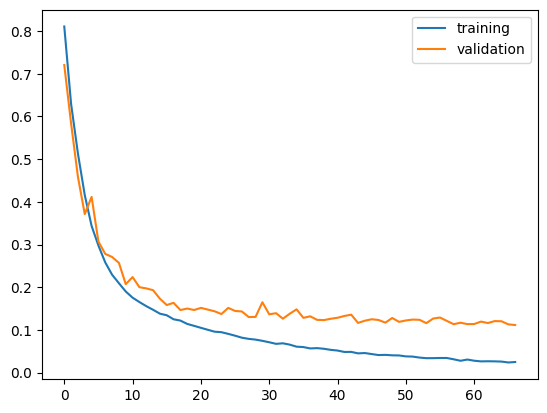
\includegraphics[width=0.8\linewidth]{./SGD.png} 
    \caption{Training error and Validation error of SGD.}
    \label{figure:sample figure} % assign a unique label to each figure
\end{figure}

\section{Averaged Stochastic Gradient Descent}

\begin{figure}[h]
    \centering % figure is centered on the page
        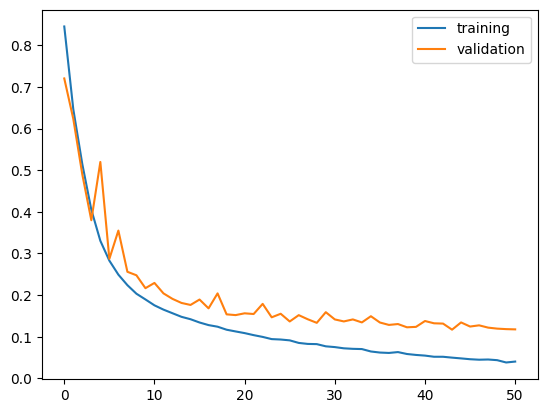
\includegraphics[width=0.8\linewidth]{./ASGD.png} 
    \caption{Training error and Validation error of ASGD.}
    \label{figure:sample figure} % assign a unique label to each figure
\end{figure}

\section{Adam algorithm}

\begin{figure}[h]
    \centering % figure is centered on the page
        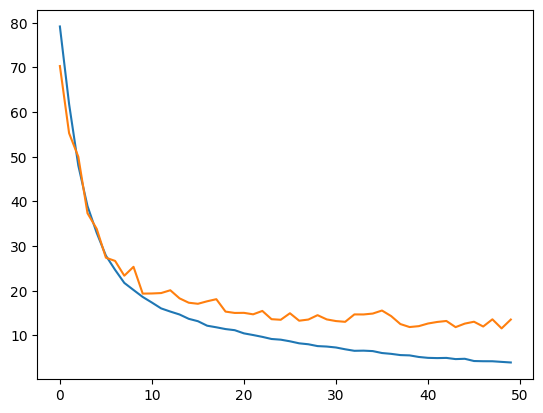
\includegraphics[width=0.8\linewidth]{./ADAM.png} 
    \caption{Training error and Validation error of Adam.}
    \label{figure:sample figure} % assign a unique label to each figure
\end{figure}

\section{Adamw algorithm}
\begin{figure}[h]
    \centering % figure is centered on the page
        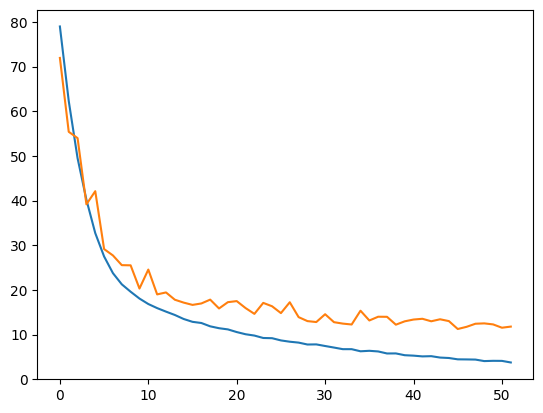
\includegraphics[width=0.8\linewidth]{./ADAMW.png} 
    \caption{Training error and Validation error of Adamw.}
    \label{figure:sample figure} % assign a unique label to each figure
\end{figure}

% \begin{table}[h]
%     \centering % table is centered on the page
%     \caption{This is how you make a table.} % The caption of the table is defined here
%     \label{table:sample table} % Assign a unique label to each table
%     \begin{tabular}{llcr} 
%         \toprule
%             & \textbf{parameter} & \textbf{type 1} & \textbf{type 2}\\
%         \midrule
%             $k_{0}$  & something     & $x$           & $y$\\
%             $k_{0}$  & other thing   & $E = mc^2$    & $z$\\ 
%             $\tau$   & exponent      & 2             & 3 \\
%         \bottomrule
%     \end{tabular}
% \end{table}




\chapter{Conclusion}

\chapter{Acknowledgements}

This report is done by both authors with tasks being shared in an equal fashion. Shuohui is in charge of both designing and running the training model and visualizing the data structure, while Yujie is primarily in charge of research for novel algorithms and providing ideas for the project.

\chapter{Reference}

1.The Implicit Bias of Gradient Descent on Separable Data \\
2.Characterizing Implicit Bias in Terms of Optimization Geometry \\
3.Stability vs Implicit Bias of Gradient Methods on Separable Data and Beyond \\
4.Implicit Bias of Gradient Descent for Mean Squared Error Regression with Two-Layer Wide Neural Networks \\
